Assuming the physics models\cite{miha, bart} for the drift of the charge carriers in germanium detectors and their input parameters taken from the measurements\cite{miha, bart} are precise enough the simulation based on them still needs to be tuned for each individual detector or at least for a series of similar detectors. This is because the pulse shape is affected by many things, such as the impurity density and the surface treatment of the detector, the electronics system connected, etc. These properties vary in different detector systems. Several data samples were taken with the first GERDA Phase II prototype detector Siegfried I (see Sec.~\ref{sec:gerda:stat3}) and its teststand (see Sec.~\ref{sec:tt:comc}) to characterize the detector. Simulation was verified with these data sets. The results are described in this chapter.

\section{Detector characterization measurements}
\label{sec:psa:char}
Detailed description of the characterization measurements with Siegfried I is available in Ref.~\cite{Sie07}. Data samples used to verify the simulation were taken in the following two measurements:
\begin{description}
\item[Surface scanning:] The surface of segment 13, 14 and 15 of Siegfried I (see Fig.~\ref{fig:ger:segm} for the segmentation naming scheme) was scanned in $\phi$ (azimuth angle) direction using a 75~kBq $^{152}$Eu source inside a copper collimator with a length of 52~mm and a pin-hole diameter of 1~mm. The spot size on the detector surface was estimated to be 150~mm$^{2}$, where the distance between the collimator and the detector was 50~mm. The spot was pointed at $z = 0$ (see Fig.~\ref{fig:pss:coo} for the coordinate system). The step size of the scanning was chosen to be 5$^{\circ}$ in segment 14 and 10$^{\circ}$ in segment 13 and 15. An uncertainty in $\phi$ of $\Delta \phi=2.5^{\circ}$ was estimated. In total 25~measurements were performed so that 180$^{\circ}$ azimuth angle was covered. The pulses of the core and all segments were recorded for each measurement. There were about $50\ 000$~events per measurement.
\item[Occupancy measurement:] A 60~kBq $^{60}$Co source was positioned about 15~cm above the center of Siegfried I (see Fig.~\ref{fig:ph:occ}). The energy deposits seen by each segment and the core were recorded.
\end{description}

The 122~keV $\gamma$ line from the $^{152}$Eu source was used to study the drift of the electrons. Because these low energy photons cannot penetrate too much into germanium and mostly deposit energy locally by photoelectric effect (see Sec.~\ref{sec:det:gamma}), they create electron-hole pairs mainly near the outer surface of the detector. The holes reach the outer surface almost immediately, while the electrons have to drift through nearly the whole bulk of the detector until they reach the inner surface. The shapes of the pulses recorded with the core of the detector are hence mainly affected by the drift of the electrons. 

To analyze the pulse shapes quantitatively the 10\%-30\% and 10\%-90\% risetimes of the core pulses were calculated. Figure~\ref{fig:psa:rt10} shows the average risetimes as a function of the azimuth angle $\phi$. The dashed lines indicate the segment boundaries. Clear oscillation patterns can be seen in both cases. This indicates a longitudinal anisotropy of the drift velocities of electrons in different $\phi$ angles because they need different time to drift through nearly the same distance.\footnote{Strictly speaking, because of the bend of the drift trajectories the distances covered by electrons in different $\phi$ angles are sightly different from each other. However, this is a second-order effect. The difference of the risetimes is mainly caused by the different drift velocity along $r$ in different $\phi$ angles.}

\begin{figure}[htbp]
\centering
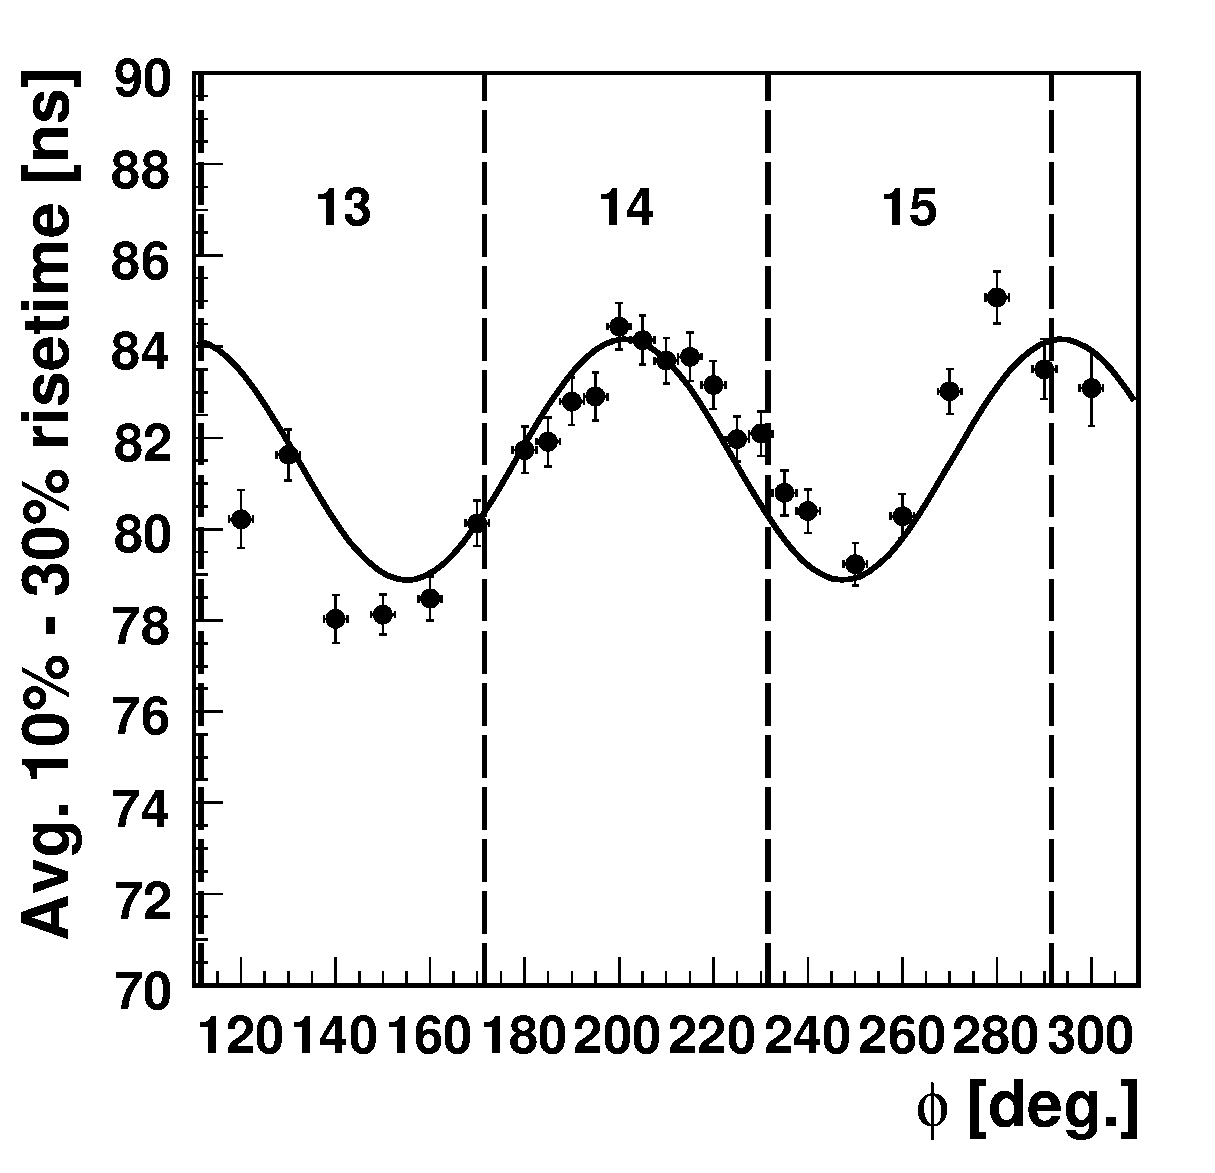
\includegraphics[width=0.45\textwidth]{phi_risetime1030}
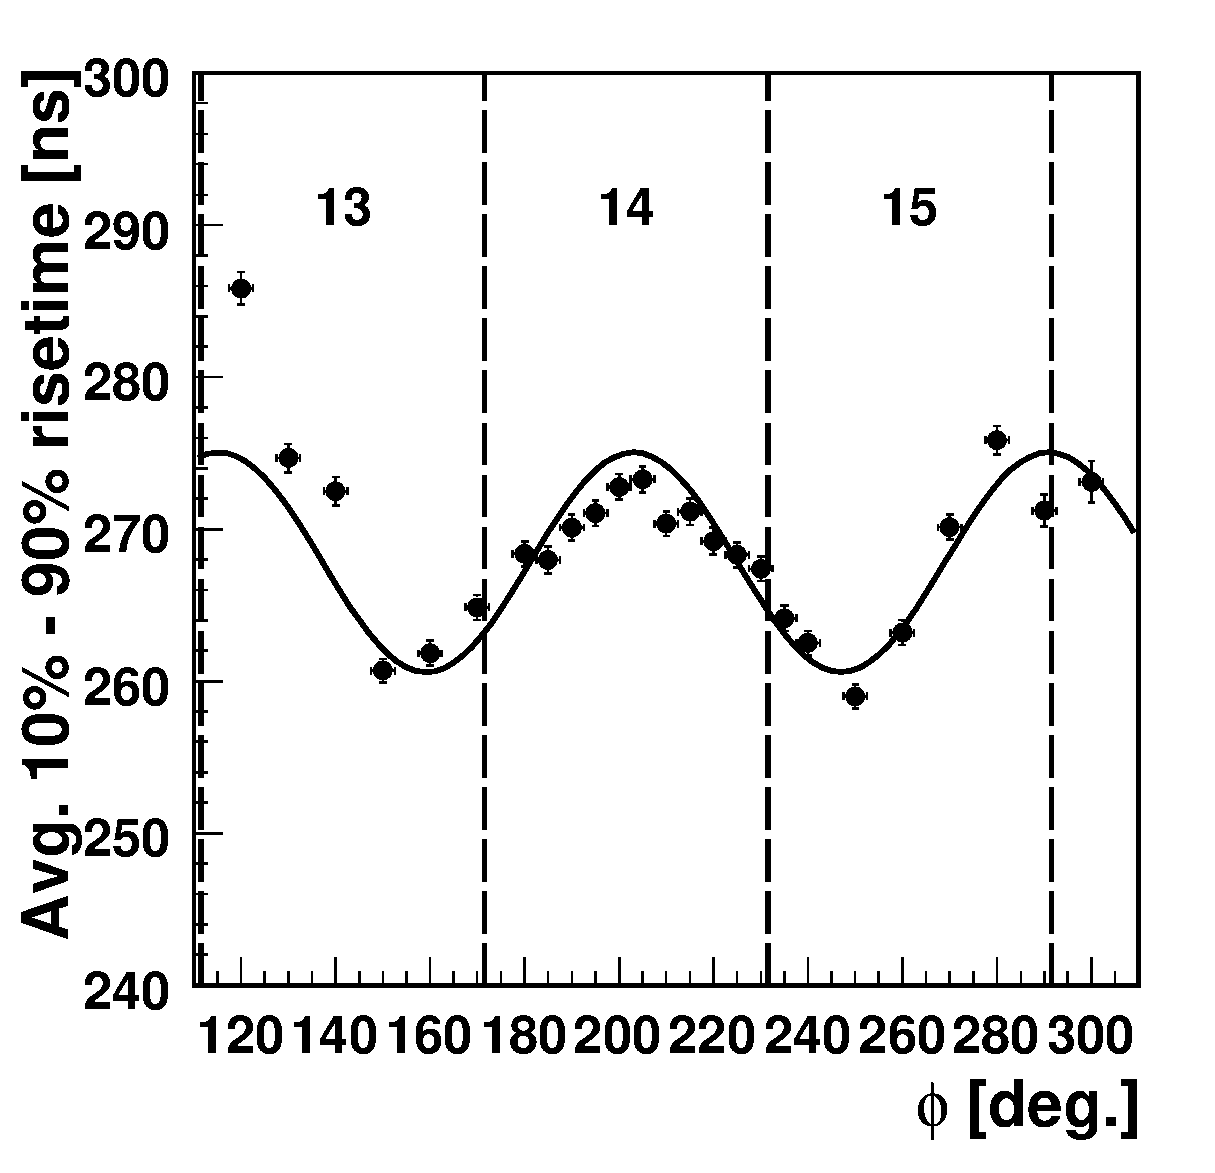
\includegraphics[width=0.45\textwidth]{phi_risetime1090}
\caption{Average 10\%-30\% (left) and 10\%-90\% (right) risetimes of the core pulses as a function of the azimuth angle $\phi$ (taken from Ref.~\cite{Sie07}).}
\label{fig:psa:rt10}
\end{figure}

The fits with a sine function (solid lines in Fig.~\ref{fig:psa:rt10}) gave periods of about 90$^{\circ}$ for the longitudinal anisotropy of the drift of electrons. This feature can be explained by the model introduced in previous chapter and revealed in Fig.~\ref{fig:pss:trjs}. Direct comparison of the pulse shapes between data and simulation is described in Sec.~\ref{sec:psa:lon}

The result of the occupancy measurement is shown in Fig.~\ref{fig:ph:mcb}. Different occupancies of segments in the same layer indicate the transverse anisotropy of the drift of charge carriers, namely, the bend the drift trajectories. This can also be explained by the models introduced in the previous chapter and revealed in Fig.~\ref{fig:pss:trjs}. Detailed comparison of the occupancy distribution between data and simulatioin is described in Sec.~\ref{sec:psa:tra}

\section{Longitudinal anisotropy}
\label{sec:psa:lon}
Pulse induced in the core electrode by the drift of electrons from outer surface to the inner surface of Siegfried I was simulated. The geometry, the operation voltage and the impurity density were implemented in the simulation according to the values listed in Table~\ref{tab:tt:detpar}. Figure~\ref{fig:psa:rt10} shows that the $\langle 110 \rangle$ axis of Siegfried I, along which electrons drift slowest hence the risetimes reach the maxima, was nearly aligned with the right boundary of segment 15, \textit{i.e.}, $\phi_{110} \approx 0$ (see Fig.~\ref{fig:pss:coo}). This was also implemented in the simulation. The decay time of 50~$\mu$s and the cut-off bandwidth of 37.5~MHz was implemented according to the specification of the electronics system. The electric noise was not added to the simulated pulse so that it can be used as a smooth fitting function with three free parameters: the \emph{Amplitude}, the \emph{Time offset} of the pulse and the \emph{Time scale} factor, a number multiplied to the time stamp of each sampling point of the pulse to stretch or squeeze the pulse in time.

The simulated pulse induced by the drift of electrons along the $\langle 110 \rangle$ axis was used to fit to each pulses from the scanning data. Figure~\ref{fig:psa:s2d} shows one of the fits. The dots with error bars are the sampling points of the pulse from data. The error was set according to the noise level.

\begin{SCfigure}[][htbp]
\centering
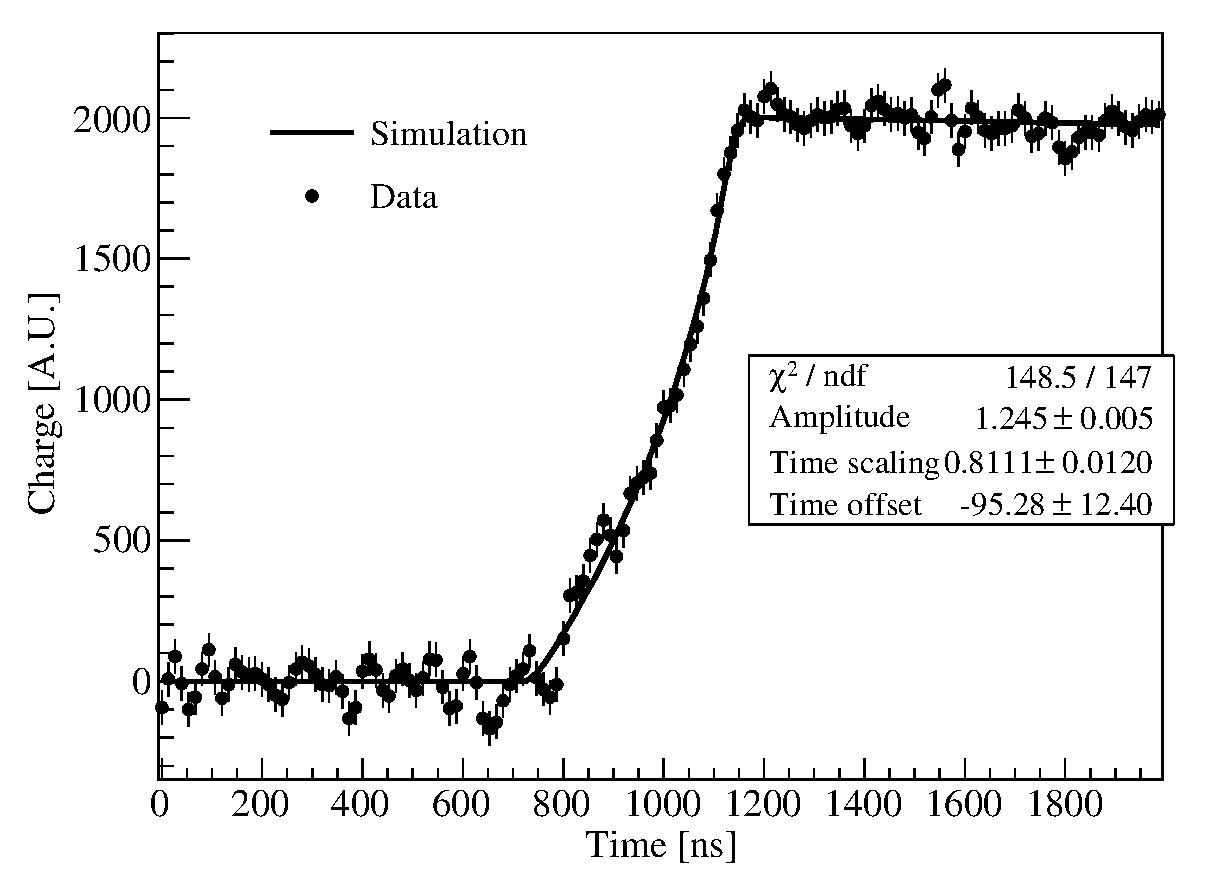
\includegraphics[width=0.5\textwidth]{PSs2d}
\caption{Fit of simulated pulse to a real one. The error bars of the sampling points are set according to the noise level.}
\label{fig:psa:s2d}
\end{SCfigure}

If the risetime of the simulated pulse is the same as the pulse from data, the free parameter \emph{Time scale} determined by the fitting should be equal to one. A value smaller than one indicates that the simulated pulse is longer than in reality; a value larger than one indicates that the simulated pulse is shorter than in reality. The time scale given in Fig.~\ref{fig:psa:s2d} shows that the simulated pulse is about 20\% longer than the pulse chosen from data.

The $\chi^{2}$ and three parameters from the fits to all the pulses in each scanning data set taken in a certain $\phi$ angle were recorded. Fits with reasonable $\chi^{2}$, amplitude and time offset were chosen for the later analysis. The time scale distribution of the chosen sub data set was fitted with a Gaussian function. The mean values are plotted in Fig.~\ref{fig:psa:tsc} as the black dots. The width of the Gaussian function are taken as the error bar.

\begin{figure}[htbp]
\centering
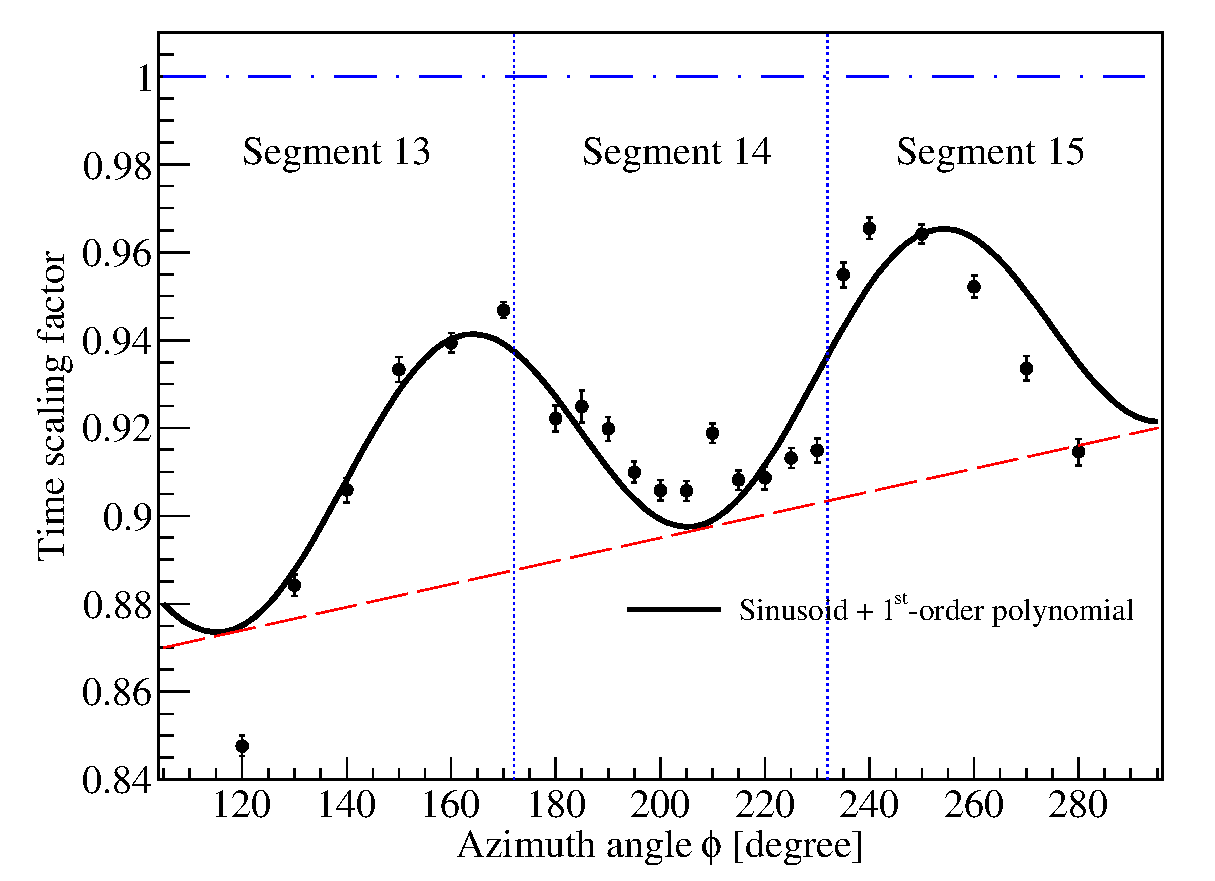
\includegraphics[width=0.6\textwidth]{tsc}
\caption{Mean time scale (black dots) obtained from the fits of one simulated pulse to those from the scanning data. The distribution was fitted with a sine wave plus a 1$^{st}$-order polynomial. The period of the sine wave was fixed to $90^{\circ}$. The baseline of the oscillation pattern shown as the dashed line in the plot changes with $\phi$ and systematically deviates from one about 10\%.}
\label{fig:psa:tsc}
\end{figure}

The mean time scale as a function of the azimuth angle $\phi$ shows similar oscillation pattern as the risetime distributions shown in Fig.~\ref{fig:psa:rt10}. However, the baseline of the pattern shown as the dashed line in Fig.~\ref{fig:psa:tsc} changes with $\phi$ and systematically deviates from one. The deviation is about 10\% on average. One possible explanation for the dependence of the baseline upon $\phi$ is that the impurity density may change with $\phi$.

The pulses corresponding to all scanning points were also simulated. They were compared to their counterparts in data using the same method. The distribution of the mean time scales is shown in Fig.~\ref{fig:psa:tsl}. The baseline obtained in Fig.~\ref{fig:psa:tsc} is overlayed to guide the eye. The system deviation from one can be easily corrected using the baseline as a correction function. After the correction the deviation is around 3\%.

\begin{figure}[htbp]
\centering
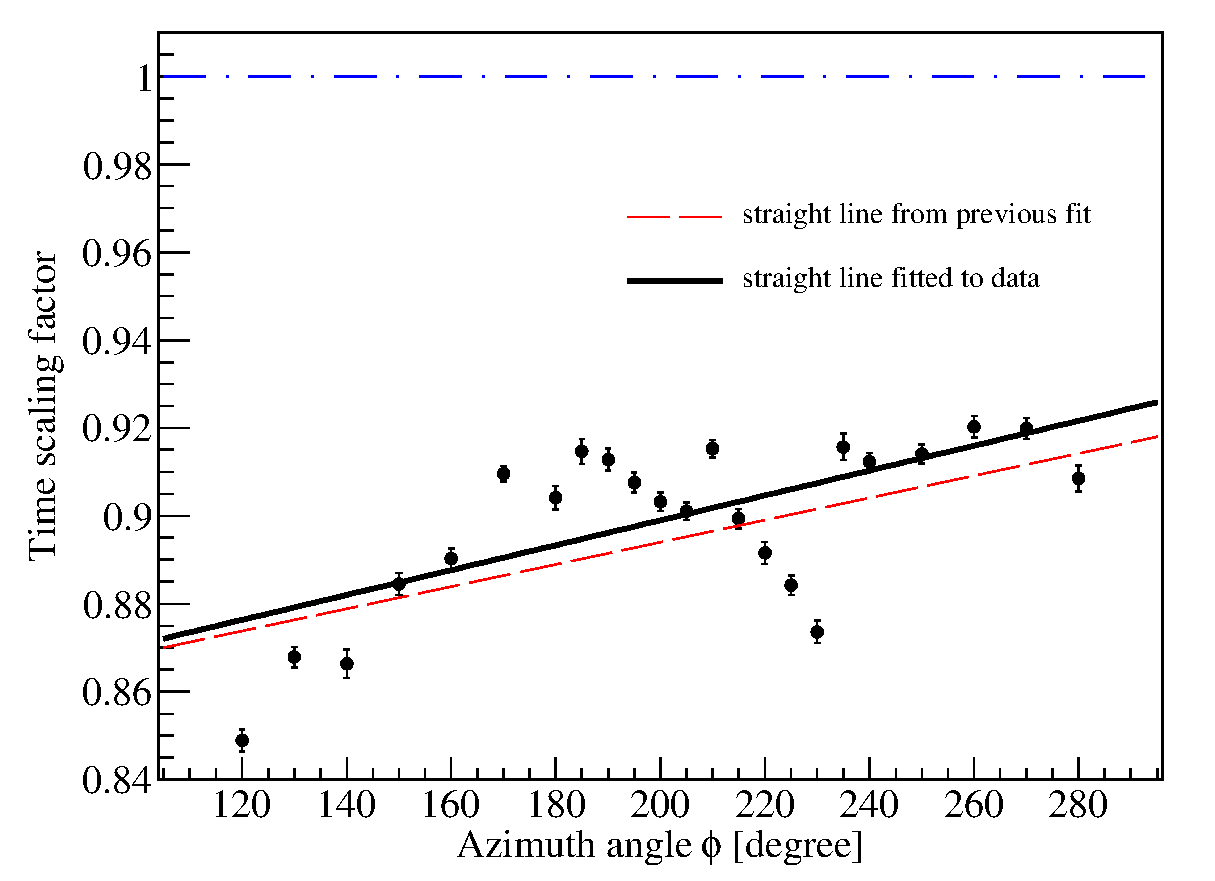
\includegraphics[width=0.6\textwidth]{tsline}
\caption{Mean time scale (black dots) obtained from the fits of simulated pulses to their counterparts from the scanning data. The baseline obtained in Fig.~\ref{fig:psa:tsc} is overlayed to guide the eye.}
\label{fig:psa:tsl}
\end{figure}


\section{Transverse anisotropy}
\label{sec:psa:tra}
The transverse anisotropy of the drift leads to the bend of the drift trajectories as shown in Fig.~\ref{fig:pss:trjs}. Consequently, the charge carriers created in a segment may drift into its neighboring segment. Some segments would always see more events than others if the trajectories are more likely to bend to it. The occupancy of each segment, namely, the number of events recorded by the segment, is hence different. This is shown in Fig.~\ref{fig:ph:mcb}. Detailed studies show that this feature is independent of the energy deposited.

To verify how well this feature can be simulated $100\ 000$ hits with the same energy were homogeneously distributed in the middle layer of Siegfried I. The drift of holes created by each hit were simulated. If a trajectory ends on the outer surface of one segment, the number of events seen by that segment increases by one. 

The simulated occupancy distribution was compared to data as shown in the left plot of Fig.~\ref{fig:psa:focc}. It changes with $\phi_{110}$, the angle between the segment boundary and the crystal axis (see Fig.~\ref{fig:pss:coo}). The difference of the distributions between data and simulation changes with $\phi_{110}$ consequently. This is shown in the right plot of Fig.~\ref{fig:psa:focc}. The difference is defined as a value proportion to $\sum_{i=1}^{6} (N_{i}^{sim}-N_{i}^{dat})$ where $N_{i}^{sim}$ and $N_{i}^{dat}$ are the numbers of events in segment $i$ for simulation and data, respectively.

\begin{figure}[htbp]
\centering
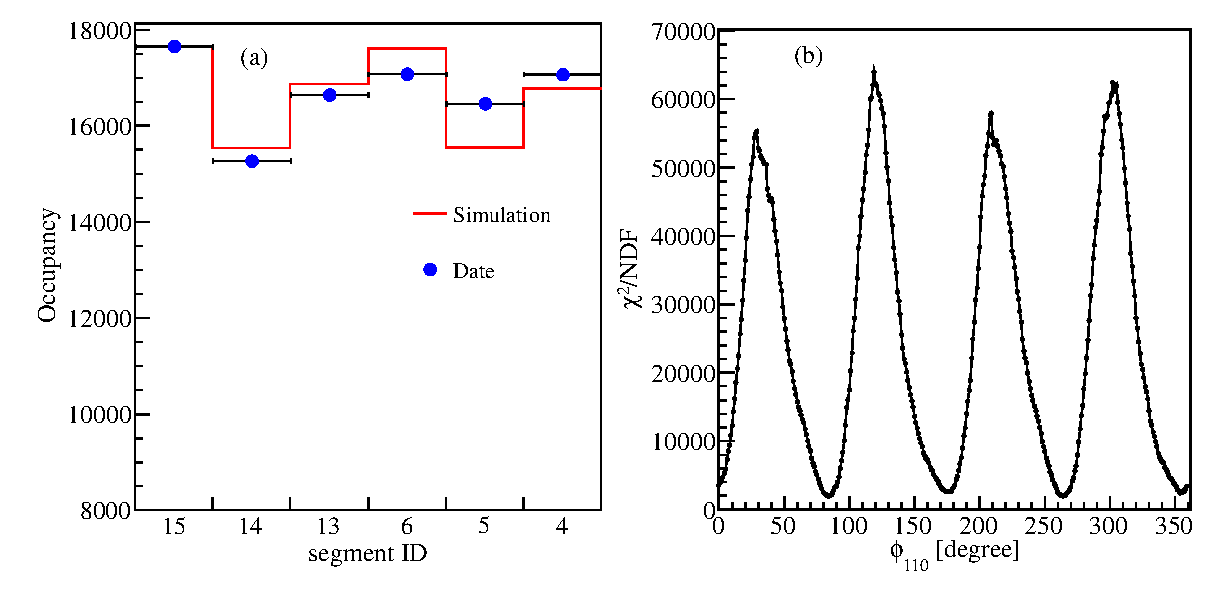
\includegraphics[width=\textwidth]{fitocc}
\caption{Left: comparison of the occupancy distribution between data and simulation. Right: difference of the two distributions as a function of $\phi_{110}$, the angle indicating the orientation of the crystal axis with respect to the segment boundary.}
\label{fig:psa:focc}
\end{figure}


\section{Summary}
\label{sec:psa:sum}

both indicate anisotropy of the impurity distribution along r.

%%% Local Variables:
%%% mode:latex
%%% TeX-master: "thesis"
%%% End:
